\documentclass[10pt]{article}

% Packages
\usepackage[left=1.75cm,right=1.75cm,top=2cm,bottom=2cm]{geometry}
\usepackage{amsmath, amssymb}
\usepackage{graphicx}
\usepackage{csvsimple}
\usepackage{caption}
\usepackage{subcaption}
\usepackage{enumitem}
\usepackage{hyperref}
\usepackage{fancyhdr}
\usepackage{titlesec}
\usepackage{etoolbox}
\usepackage{makecell} % For multi-line headers#
\usepackage{adjustbox}
\usepackage[table]{xcolor}
\usepackage{csvsimple}
\usepackage{array}
\usepackage{booktabs}
\usepackage{caption}
\usepackage{siunitx}
\usepackage{ragged2e}
\usepackage{blindtext}

% Header/Footer
\pagestyle{fancy}
\fancyhf{}
\rhead{ML Project Report: Fake News Detection}
\lhead{Martin Wagner, Philipp Hoffmann}
\cfoot{\thepage}

% Section formatting
\titleformat{\section}{\large\bfseries}{\thesection}{1em}{}
\titleformat{\subsection}{\normalsize\bfseries}{\thesubsection}{1em}{}

% Title
\title{\textbf{Machine Learning Project Report: Fake News Detection}}
\author{Martin Wagner, Philipp Hoffmann \\
	Applied ML – Ludwig-Maximilians-Universität München \\
	\texttt{\href{mailto:wagner.mar@campus.lmu.de}{wagner.mar@campus.lmu.de},
	\href{mailto:philipp.hoffmann@campus.lmu.de}{philipp.hoffmann@campus.lmu.de}}}
\date{\today}



\begin{document}
	
	\maketitle
	
	\section{Task Overview}
	Briefly describe the dataset or model you worked on, the goal of the project, and why the task is challenging. For example, challenges may include complex preprocessing, large dataset size, class imbalance, poor performance of baseline approaches, or the need for more complex models to achieve good results.
	
	\blindtext
	
	\section{Methods}
	We compared the performance of logistic regression and linear svm models (mainly on the collection of titles) using different vectorization techniques from natural language processing. 
	We used \texttt{TfidfVectorizer} and \texttt{CountVectorizer} from \texttt{scikit-learn} for basic text vectorization. Given a vocabularly of tokens (e.g. words), bag-of-words assigns to a document $d$ for each token $t$, the term-frequency $\operatorname{tf}(t,d)$, defined as the count of term $t$ in $d$ divided by the total number of terms. A bit more evolved is Tf-Idf-vectorization, which also takes into account the frequency of how often a term occurs in a fixed corpus $D=\{d_1, \dots, d_n\}$ of documents $d_1, \dots, d_n$. Given a term $t$, the inverse-document frequency of $t$ in $D$ is $\operatorname{idf}(t,D):=1+\log\left(\frac{1+n}{1+\operatorname{df}(t)}\right)$, where $\operatorname{df}(t)$ is the number of documents in $D$ containing the term $D$. Then the Tf-Idf-score of a term $t$ with respect to the collection $D$ is defined as \[\operatorname{tf-idf}(t,d,D):=\operatorname{tf}(t,d)\operatorname{idf}(t,D).\]
	Note that $d$ does not need to be contained in the collection $D$ of documents itself. The tools from \texttt{scikit-learn} also apply $L2$-normalization to the obtained vectors, which we retained. Additionally, we applied z-score normalization afterwards, as this gave us better results, in particular for linear SVMs. 
	We adopted models in courselib to support sparse matrix calculation and implemented methods to adopt for feature shifts (due to z-score normalization) without destroying the computational efficiency resulting from the sparsity of the unshifted feature matrices. Moreover we implemented custom tokenizers using \texttt{nltk} 
	that support for example stemming or lemmatiztation, i.e. reduce words to their basic form. To test all of these options more compactly, we implemented a multi-column-vectorizer which supports vectorization of text data of one or multiple columns of a dataframe with different vectorization options.
	
	\section{Experiments and Results}
	Present your results. Use figures, tables, and metrics:
	\blindtext
	\begin{figure}[htbp]
		\centering
		\begin{subfigure}[b]{0.37\textwidth}
			\includegraphics[height=5cm]{figures/model_comparison_accuracy_evolution.pdf}
			\caption{}
			\label{fig:a}
		\end{subfigure}
		\hfill
		\begin{subfigure}[b]{0.2\textwidth}
			\includegraphics[height=5cm]{figures/model_comparison_confusion_matrices.pdf}
			\caption{}
			\label{fig:b}
		\end{subfigure}
		\hfill
		\begin{subfigure}[b]{0.37\textwidth}
			\includegraphics[height=5cm]{figures/vectorization_comparison_feature_number_impact.pdf}
			\caption{}
			\label{fig:c}
		\end{subfigure}
		\caption{figure}
		\label{fig:comparison}
	\end{figure}
		\begin{table}[htbp]
		\centering
		\small
		\setlength{\tabcolsep}{4pt}
		\renewcommand{\arraystretch}{1.1} % Increase row height for better spacing
		
		\label{tab:results2}
		\begin{adjustbox}{scale=.8}
			\rowcolors{2}{lightgray}{white} % Alternate row colors
			\begin{tabular}{|l|l|l|r|r|r|r|r|}
				\hline
				\rowcolor{gray!30} % Header background color
				\bfseries Model & \bfseries batch size & \bfseries  \makecell{Train\\Accuracy\\{\footnotesize[\%]}} & \bfseries  \makecell{Test\\Accuracy\\{\footnotesize[\%]}} & 
				\bfseries  \makecell{Training\\Time\\{\footnotesize[s]}} & 
				\bfseries Precision & \bfseries Recall & \bfseries F1-Score \\
				\hline
				\csvreader[
				late after line=\\\hline
				]{tables/model_comparison_table.csv}{}%
				{\csvcoli & \csvcolii & \csvcoliii & \csvcoliv & \csvcolv & \csvcolvi & \csvcolvii & \csvcolviii}%
			\end{tabular}
		\end{adjustbox}
		\vspace{0.2cm}
		\caption{table}
	\end{table}
	
	\blindtext
		\begin{table}[htbp]
		\centering
		\small
		\setlength{\tabcolsep}{4pt}
		\renewcommand{\arraystretch}{1.1} % Increase row height for better spacing
		
		\label{tab:results}
		\begin{adjustbox}{scale=.8}
			\rowcolors{2}{lightgray}{white} % Alternate row colors
			\begin{tabular}{|l|l|l|r|r|r|r|r|r|r|}
				\hline
				\rowcolor{gray!30} % Header background color
				\bfseries Vectorization & \bfseries Stop Words & \bfseries Tokenizer & \bfseries Features & 
				\bfseries \makecell{Train\\Accuracy\\{\footnotesize[\%]}} & 
				\bfseries \makecell{Test\\Accuracy\\{\footnotesize[\%]}} & 
				\bfseries Precision & \bfseries Recall & \bfseries F1-Score & 
				\bfseries \makecell{Vectorization\\Time\\{\footnotesize[s]}} \\
				\hline
				\csvreader[
				late after line=\\\hline
				]{tables/vectorization_comparison_table.csv}{}%
				{\csvcoli & \csvcolii & \csvcoliii & \csvcoliv & \csvcolv & \csvcolvi & \csvcolvii & \csvcolviii & \csvcolix & \csvcolx}%
			\end{tabular}
		\end{adjustbox}
		
		\vspace{0.2cm}
		\caption{table}
	\end{table}
	
	\blindtext


		\begin{table}[htbp]
		\centering
		\small
		\setlength{\tabcolsep}{4pt}
		\renewcommand{\arraystretch}{1.1}
		
		
		\begin{adjustbox}{scale=.8}
			\rowcolors{2}{lightgray}{white}
			\begin{tabular}{|l|l|r|r|r|r|}
				\hline
				\rowcolor{gray!30} % Header background color
				\bfseries  \makecell{n-gram\\range} & 
				\bfseries  Features & 
				\bfseries  \makecell{Train\\Accuracy\\{\footnotesize[\%]}} & 
				\bfseries  \makecell{Test\\Accuracy\\{\footnotesize[\%]}} & 
				\bfseries \makecell{Vectorization\\Time\\{\footnotesize[s]}}&
				\bfseries  \makecell{Training\\Time\\{\footnotesize[s]}} \\
				\hline
				\csvreader[
				late after line=\\\hline
				]{tables/comparison_ngrams.csv}{}%
				{\csvcoli & \csvcolii & \csvcoliii & \csvcoliv & \csvcolv & \csvcolvi}%
			\end{tabular}\end{adjustbox}
		\caption{table}
	\end{table}
	
	\begin{table}[htbp]
		\centering
		\small
		\setlength{\tabcolsep}{4pt}
		\renewcommand{\arraystretch}{1.1} % Increase row height for better spacing
		

		\begin{adjustbox}{scale=.8}
		\rowcolors{2}{lightgray}{white}
		\begin{tabular}{|l|l|r|r|r|r|r|}
			\hline
			\rowcolor{gray!30} % Header background color
			\bfseries  Data & 
			\bfseries  Features & 
			\bfseries  \makecell{Train\\Accuracy\\{\footnotesize[\%]}} & 
			\bfseries  \makecell{Test\\Accuracy\\{\footnotesize[\%]}} & 
			\bfseries \makecell{Vectorization\\Time\\{\footnotesize[s]}}&
			\bfseries  \makecell{Training\\Time\\{\footnotesize[s]}} \\
			\hline
			\csvreader[
			late after line=\\\hline
			]{tables/vectorization_more_text_data.csv}{}%
			{\csvcoli  & \csvcoliii & \csvcoliv & \csvcolv & \csvcolvi & \csvcolvii}%
		\end{tabular}
		\end{adjustbox}
		\vspace{0.2cm}
		\caption{Table}
	\end{table}
	
	\blindtext 
	\begin{figure}
		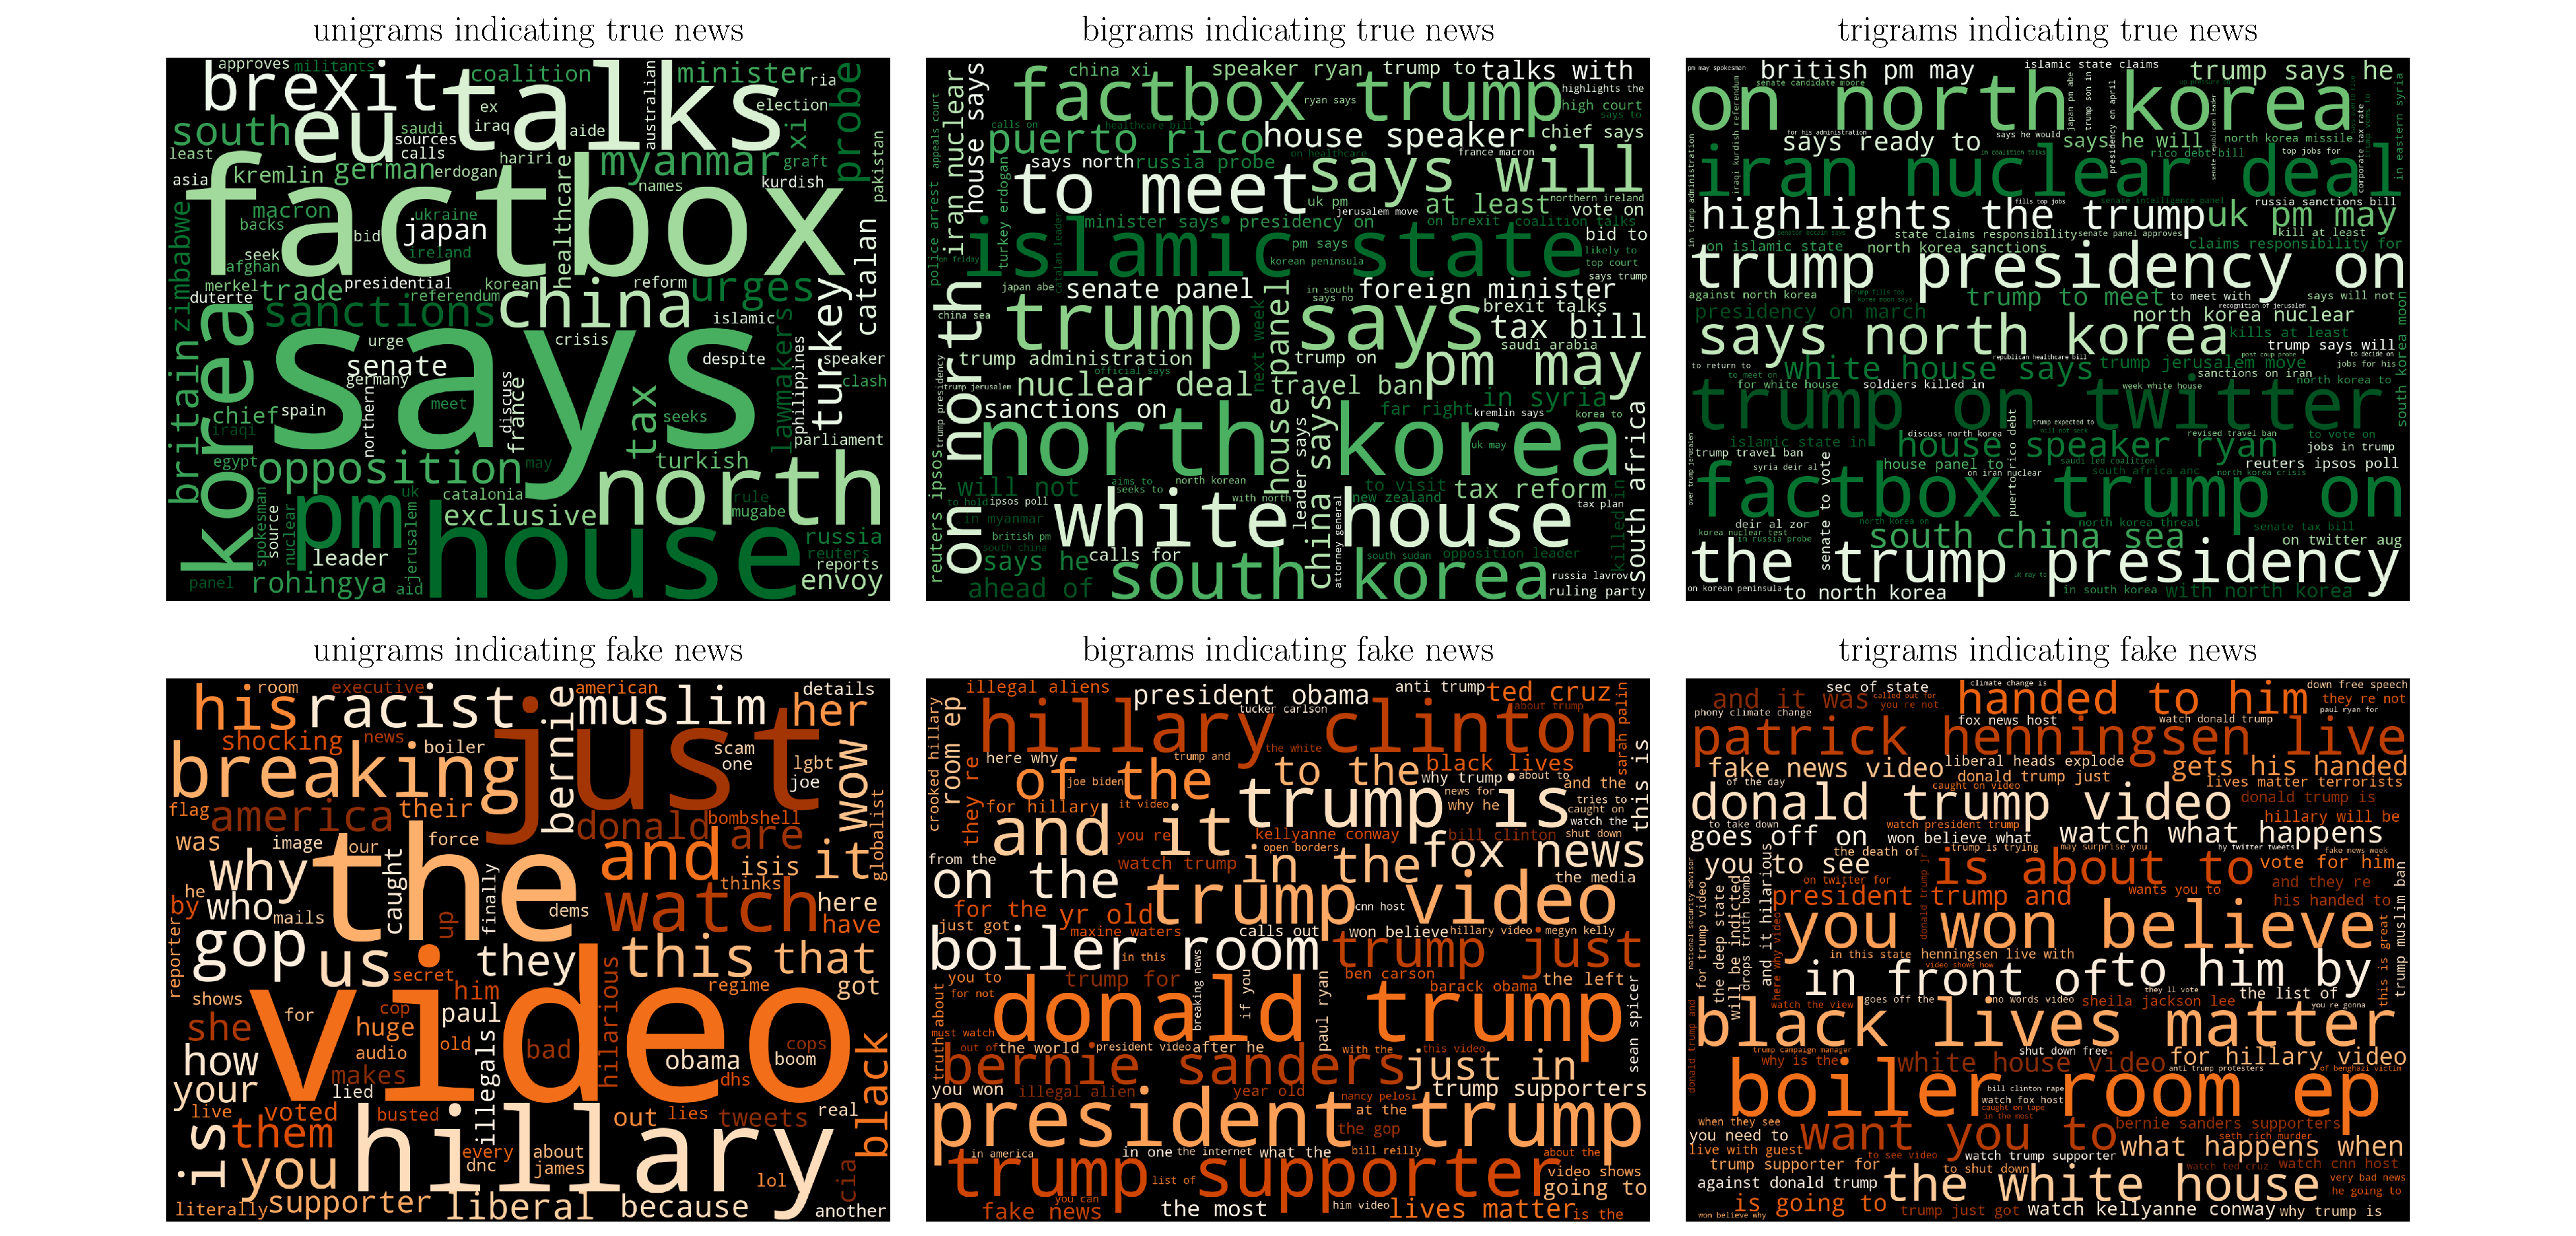
\includegraphics[width=\textwidth]{figures/wordclouds.pdf}
		\caption{figure}
	\end{figure}
	

	
	
	\section{Discussion}
	Summarize key findings, insights, or issues. Optionally, suggest future work or limitations.
	\blindtext
	
\end{document}